\documentclass{article}
\usepackage[utf8]{inputenc}
\usepackage[english]{babel}
\usepackage{graphicx}
\usepackage[dvipsnames]{xcolor}
\usepackage{amsfonts}

\def\warning#1{\color{red} #1 \color{black}}
\def\note#1{\color{cyan} #1 \color{black}}
\def\acca#1{\color{OliveGreen} #1 \color{black}}
\def\accb#1{\color{Lavender} #1 \color{black}}
\def\accc#1{\color{Violet} #1 \color{black}}
\def\circled#1{\raisebox{.5pt}{\textcircled{\raisebox{-.9pt} {#1}}}}

\graphicspath{{./img/}}

\begin{document}

\title{Hoe los ik een examen Discrete Wiskunde op?}
\date{}
\author{}
\maketitle

\tableofcontents


Het examen Discrete Wiskunde verandert weinig en bestaat altijd uit zeven vragen. Zes van deze vragen zijn analoog met elke examenperiode en één vraag is willekeurig vanuit heel de cursus. In dit document wil ik technieken toelichten om het examen op een goede manier op te lossen. Dit gaat vooral over trukjes in Excel en de Antiview die je kan gebruiken in plaats van alles manueel te doen. 

\section{Velden}
\subsection{Het algoritme van Euclides}
Het algoritme van Euclides komt altijd terug dus dit moet heel goed gekend zijn. Het is nuttig om Excel het meeste werk te laten doen. Stel dat we 97 willen delen door 53. Je begint met de startopstelling.
 \begin{center}
  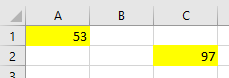
\includegraphics{euclidische_deling_1}
  \label{fig:euclidische_deling_1}
 \end{center}
Daarna gebruik je de functie \texttt{FLOOR.MATH} om \warning{todo}


\subsection{Berekenen van een primitieve wortel}
Een primitieve wortel is het kleinste getal dat niet deelbaar is door een bepaald getal voor een bepaald veld. Het berekenen van een primitieve is heel eenvoudig. 
Er is slechts één gegeven nodig en dat is het veld. We nemen het volgende voorbeeld: Bereken de primitieve wortel over $\mathbb{Z}_{4051}.$

\begin{enumerate}
 \item Trek 1 af van het veldgetal en ontbindt dit in factoren. Gebruik het programma {\it factor} dat ook beschikbaar is op het examen. (Ingeven: {\sl factor 4050}) 
  $$4051 - 1 = 4050 = 2 * 3^{4} * 5^{2}$$
  Het getal 4050 wijst simpelweg op het aantal elementen in dit veld.
 \item We hebben het getal 4050 ontbonden in factoren. De bedoeling is om een excel-bestand op te maken zodat de primitieve wortel redelijk eenvoudig kan berekend worden. 
 Het excel-bestand heeft volgende opmaak:
 \begin{center}
  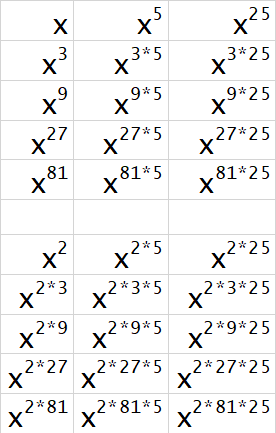
\includegraphics[height=5cm]{priem_wortel_1}
  \label{fig:priem_wortel_1}
 \end{center}

 Dit stellen allemaal delers voor van het getal 4050. Nu is het de bedoeling dat we {\sl x} vervangen door oplopende getallen startend vanaf 2. \warning{todo}
 \end{enumerate}

 
 \subsection{De baby-step, giant-step techniek}
 De baby-step, giant-step techniek wordt gebruikt om een index van een getal ten opzichte van een primitieve wortel in een bepaald veld te berekenen. Hier moet de Euclidische deling ook uitgevoerd worden dus zorg dat je dit al goed kunt. Bij dit soort vraagstukken zijn er 3 gegevens. 
 \begin{itemize}
  \item {Het veld $\mathbb{Z}$} 
  \item {Een getal in dit veld waarvan de index moet berekend worden.}
  \item {De primitieve wortel $w$}
 \end{itemize}
 Op het examen zal er staan hoe groot één giant-step moet zijn. In dit voorbeeld nemen we giant-steps die 10 baby-steps groot zijn. We beschouwen het veld $\mathbb{Z}_{71}$ en de primitieve wortel $w = 7$. We willen de index van 5 berekenen. Begin met de eerste 10 baby-steps te genereren. Je begint met de primitieve wortel, en daarna gebruik je Formule 1. De letter b stelt de n-de baby-step voor. Bekijk ook Figuur \ref{fig:babystep_giantstep_1} waarop dit gevisualiseerd staat(p. \pageref{fig:babystep_giantstep_1}).
 $$b_n = b_{n-1} * w\; \% \;71 \eqno(1)$$
 
\begin{figure}
  \begin{center}
  \caption{Voorstelling van Formule 1 voor de berekening van de baby-steps}
  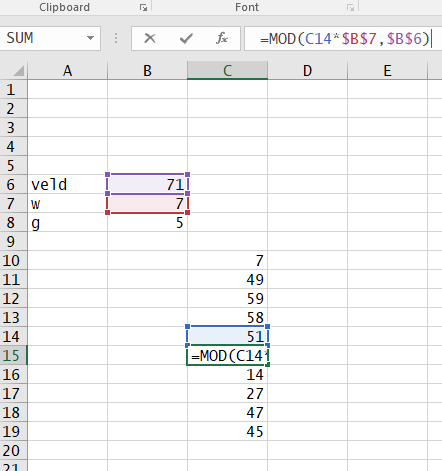
\includegraphics[width=\textwidth]{babystep_giantstep_1}
  \label{fig:babystep_giantstep_1}
  \end{center}
  
\end{figure}
  
 
Nadat de eerste 10 baby-steps genereerd zijn moet je het inverse element, ten opzichte van 71, van de laatste baby-step bepalen. Dit doe je door het algoritme van Euclides toe te passen(Figuur \ref{fig:babystep_giantstep_2}).

\begin{figure}
  \begin{center}
  \caption{Algoritme van Euclides bij de baby-step, giant-step techniek}
  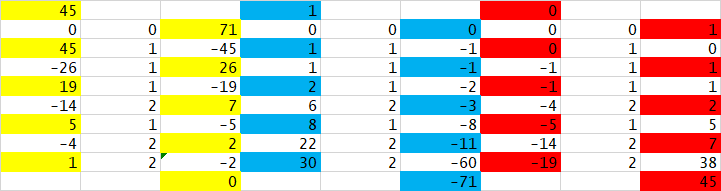
\includegraphics[width=\textwidth]{babystep_giantstep_2}
  \label{fig:babystep_giantstep_2}
  \end{center}
\end{figure}
Het inverse element is hier dus 30. Nu moeten de giant-steps gegenereerd worden. Je vertrekt vanaf het getal waarvan we de index zoeken. Daarna gebruik je Formule 1 maar vervang je de baby-step door de giant-step. Dit wordt voorgesteld in Figuur \ref{fig:babystep_giantstep_3}.


\begin{figure}
  \begin{center}
  \caption{Voorstelling van Formule 1 voor de berekening van de giant-steps}
  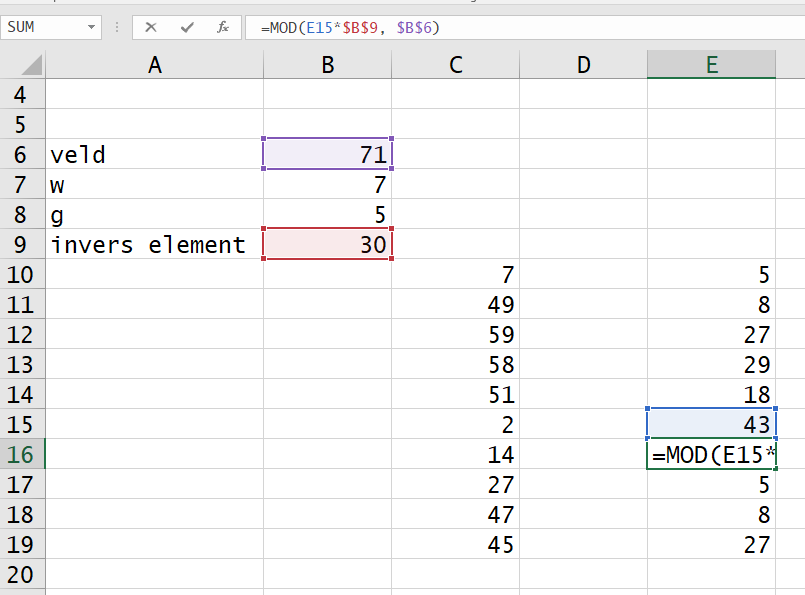
\includegraphics[width=\textwidth]{babystep_giantstep_3}
  \label{fig:babystep_giantstep_3}
  \end{center}
\end{figure}
  
Merk op dat het getal 27 zowel bij de baby-steps als bij de giant-steps voorkomt. Dit stelt de index voor die we zoeken. Het getal 27 is het achtste getal in de baby-step verzameling. Bij de giant-step verzameling is dit het derde getal. Aangezien elke giant-step een grootte heeft van tien babysteps, wordt dit nog eens vermenigvuldigd met tien. De index wordt $$8 + (3 * 10) = 8 + 30 = 38$$
De oplossing is formeel: De index van 5 over het veld $\mathbb{Z}_{71}$ met primitieve wortel $w = 7$ is 38. Er zijn 3 giant-steps en 8 baby-steps nodig.

\subsection{Irreducibele veeltermen}
Een irreducibele veelterm is een veelterm dat niet meer deelbaar is over een bepaald veld. Op het examen wordt een priemveld gegeven en een bepaalde veelterm. Beschouw het veld $F_{32}$ en de veelterm $x^5 + x^4 + 2x^3 + 2x + 1$. We weten dat $2^5 = 32$, dus $\acca{p = 2}$ en $\accc{n = 5}$. De test moet uitgevoerd worden met elke veelterm $x^{\acca{p}^{\accb{i}}} - x$ met $\accb{i} \leq \frac{\accc{n}}{2}$. Het komt erop neer dat je $n$ deelt door 2 en dit getal afrond naar beneden. Dus $floor(\frac{\accc{5}}{2}) = 2$. 

De test moet dus uitgevoerd worden met $\accb{i = 1}$ en $\accb{i = 2}$. We moeten de veelterm  dus delen door $x^{\acca{2}^{\accb{1}}} - x$ en $x^{\acca{2}^{\accb{2}}} - x$. Indien geen gemeenschappelijke deler werd gevonden dan is de veelterm irreducibel. Je kan eenvoudig de euclidische deling uitvoeren. Je moet enkel elke graad als een 'getal' zien. Zo is $4x^3 + x + 7$ gelijk aan $4017$. Onze veelterm wordt dus $112021$. \warning{in excel pls}
\begin{center}
\begin{tabular}{c c c | c c c}
 110 &  &        & 10010 &  &\\
     &  & 112021 &       &  & 112021
\end{tabular}
\end{center}



\subsection{Elliptische krommen}
Bij een vraag over een elliptische kromme krijg je zeker drie gegevens:
\begin{enumerate}
 \item Het veld en de vergelijking van de elliptische kromme
 \item De irreducibele veelterm
 \item De primitieve wortel
 \item Een groepstabel
\end{enumerate}

Op het examen worden er slides gegeven (meer specifiek, slide 6 en 10 van het bestand 1d.pptx). Dit zijn de slides waarop de berekening voor het verdubbelen van de punten opstaan, dus deze moet je niet  vanbuiten kennen. Je moet wel weten welke slide je nodig hebt, maar dit is gewoon naar de vergelijking kijken en zien welke er overeenkomt met die op de slide. Voor de verdere uitwerking van dit onderdeel worden de gegevens van het examen gebruikt.

\fbox{
  \parbox{\linewidth}{
  Beschouw het veld $F_{16}$ en de elliptische kromme $E: y^2 + xy = x^3 + \circled{3}x^2 + \circled{5}$ over dit veld. De irreducibele veelterm is $\mu = x^4 + x + 1$ en de primitieve wortel $w = x$. Gebruik de onderstaande groepstabel:
    \begin{center}
    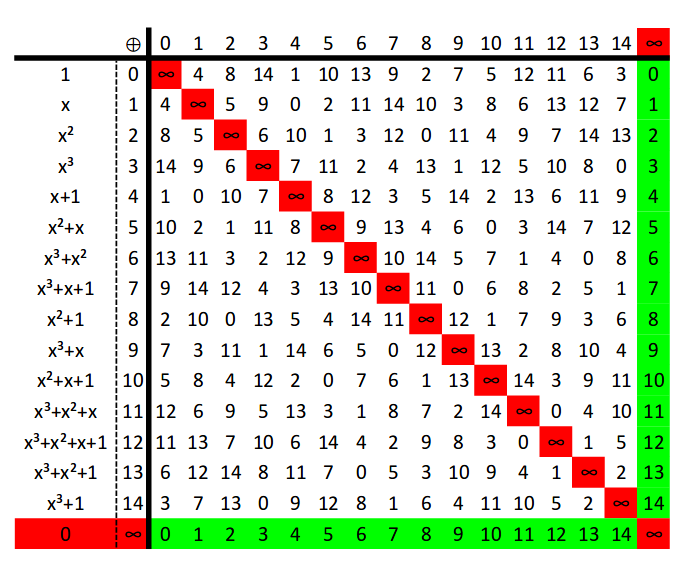
\includegraphics[width=\linewidth]{groepstabel}
    \end{center}
  }
}


\subsubsection{Berekening van de punten}
De eerste stap is altijd het berekenen van alle punten op deze elliptische kromme. 

\subsubsection{Verdubbeling van de punten}

\subsubsection{Soort bepalen}



\section{Groepen}
\subsection{Partitionering van de groepselementen in conjugatieklassen}
\subsection{Cykelindex bepalen}
Op het examen wordt er gevraagd om de cykelindex van een willekeurige drie dimensionele veelhoek te bepalen. Daarna wordt er gevraagd om het aantal configuraties te bepalen waarbij een X aantal kleuren Y maal gebruikt worden.

Op deze vraag moet de AntiView gebruikt worden die standaard al open staat op het examen met de figuur. Dit programma toont default de symmetrie en rotatie-assen niet. Zonder dit hulpmiddel is deze vraag haast onmogelijk. Je kan de assen tonen door op de knop 'Y' te drukken op het toetsenbord. In de voorbeelden gebruiken we een kubus. Je kan deze figuur ook bekomen door het programma AntiView via de commandolijn op te starten met als argument \texttt{cube}.

\begin{center}
 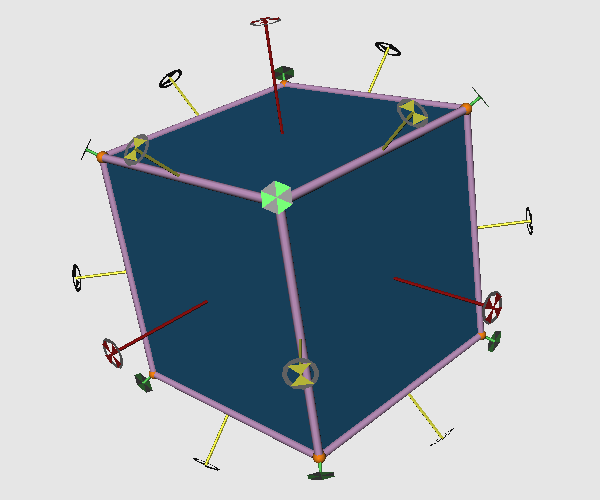
\includegraphics[width=\linewidth]{antiview_cube_1}
\end{center}

Normaal zie je 3 soorten assen verschijnen: rode, gele en groene. Elke kleur heeft zijn eigen betekenis.
\begin{itemize}
 \item \textbf{Rood}:
 \item \textbf{Geel}:
 \item \textbf{Groen}:
\end{itemize}



\end{document}
